\documentclass[12pt]{article}

\usepackage{graphicx}
\usepackage{float}
\usepackage{enumerate}
\usepackage{algorithm}
\usepackage{alltt}
\usepackage{hyperref}

\renewcommand{\ttdefault}{txtt}

\title{A Virtual Theremin Using Kinect}
\author{Niall Wingham}
\date{April 8, 2013}


\begin{document}

\maketitle

\begin{abstract}
The theremin is an electronic synthesizer that is played without being touched.  Because it gives no haptic feedback, it a natural candidate for virtualization.  In this paper we discuss our design and implementation of a virtual theremin using the Microsoft Kinect.  We demonstrate algorithms that reliably track hands and recognize simple gestures at 30 frames per second.
\end{abstract}



\section{Introduction}
A theremin consists of two perpendicular metal rods which each act as a plate in a capacitor.  The performer's hands act as the corresponding ground plates, and the hand moving to and from the rod changes the frequency of an associated oscillator.  Typically, the distance between the right hand and the vertical rod controls the pitch of the theremin while the height of left hand above the horizontal rod controls the volume.  For a video of Leon Theremin playing his invention, see \href{http://youtu.be/w5qf9O6c20o}{http://youtu.be/w5qf9O6c20o}.

\begin{figure}[H]
\caption{A \emph{Moog} Etherwave Theremin}
\centering
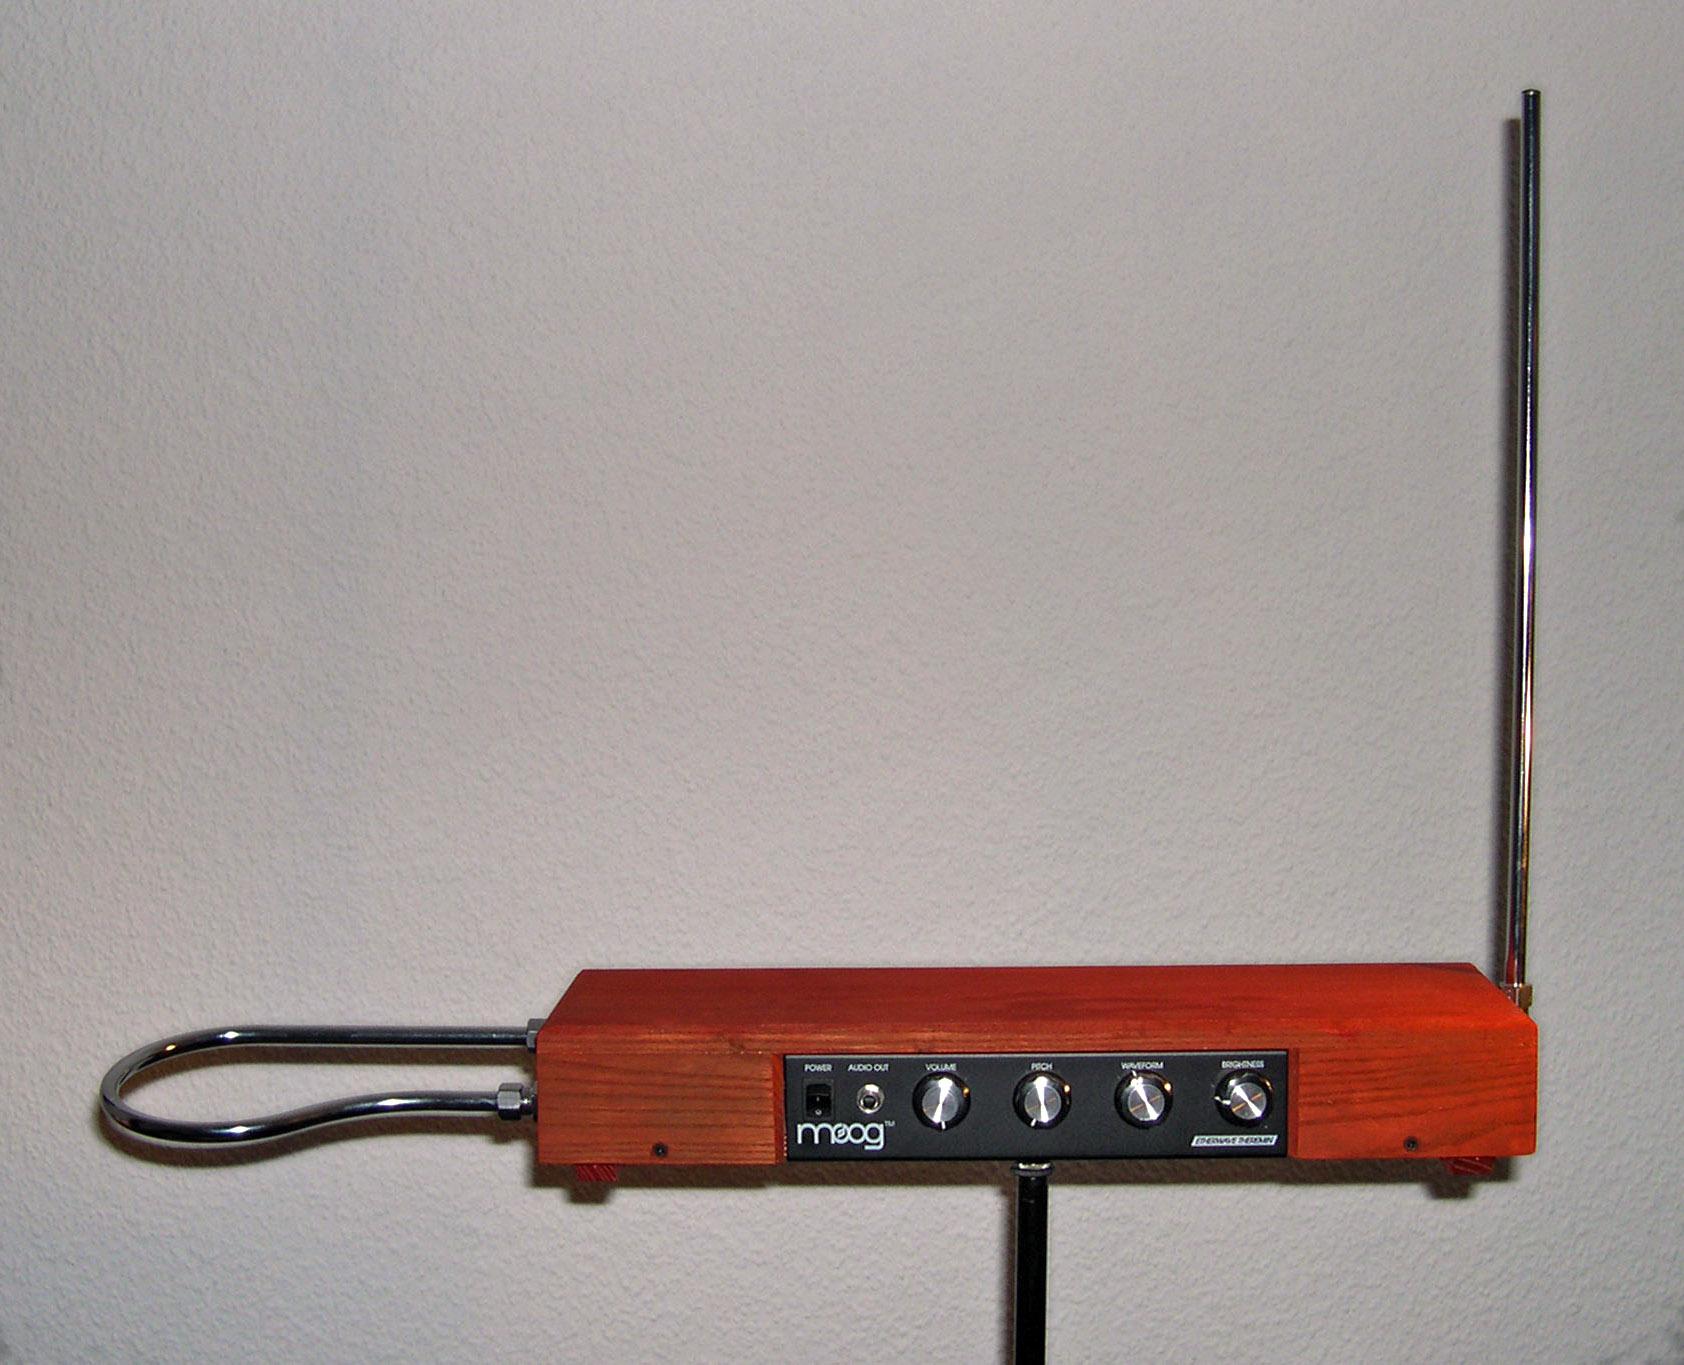
\includegraphics[width=0.33\textwidth, natwidth=1684, natheight=1365]{Etherwave_Theremin_Kit.jpg}
\end{figure}

\subsection{Motivation}
The theremin is a fascinating instrument, but it has several limitations.  Playing a theremin is quite challenging because the pitch changes over a continuous range (most instruments play only discrete pitches).  The performer needs an excellent ear to constantly ``tune" the instrument.  Theremins are also difficult to obtain: a would-be hobbyist must be willing to spend a few hundred dollars on Ebay, or be able to assemble one from a kit.  Finally, the theremin's characteristic ethereal sound is only appropriate for certain types of music.

\subsection{Objectives}
By building a virtual theremin, we aim to address each of these limitations through software.  In particular, our objectives are to:

\begin{enumerate}
\item Provide visual feedback to the performer, so it is easier to play.
\item Use only commodity hardware, so it is cheaper and more accessible.
\item Synthesize a variety of sounds, so it is more expressive.
\end{enumerate}

\subsection{Outline}
In Section 2, we introduce background material and terminology relevant to our implementation.  In Section 3, we describe the implementation of our virtual theremin.  In Section 4, we show test data and discuss the strengths and weaknesses of our algorithms.  In Section 5, we raise possibilities for future work.



\section{Preliminaries}
\subsection{Synthesizers}
A synthesizer consists of one of more voices, each of which generates sound through a chain of oscillators and effects.  A sine wave is a simple oscillator, while raising or lowering the volume is a simple effect on an oscillator.  To play a synthesized sound, each voice is sampled several thousand times per second.  An excellent introduction to synthesizers can be found \href{http://www.codeproject.com/Articles/19618/C-Synth-Toolkit-Part-I}{here}.

\subsection{Kinect}
The Microsoft Kinect provides three sets of data at each frame: a colour image, a depth image, and a skeleton image.  The colour and depth images both have pixel-coordinates, but they are slightly offset from each other due to the relative position of the cameras on the device.  The skeleton exists in real X,Y,Z space and consists of joints such as \texttt{HandLeft} or \texttt{HipCenter}.  The Kinect provides methods for transforming points between these three sets of coordinates.  More information on the Kinect can be found \href{http://www.microsoft.com/en-us/kinectforwindows/develop/resources.aspx}{here}.

\subsection{Pseudocode}
Our project is implemented in C\#, and we often make use of its functional-style LINQ methods, so it will help to be familiar with them.  For example, \texttt{[1..100].Where(Even).Take(5)} would return the (lazily generated) list \texttt{[2,4,6,8,10]}.  In the context of a function that returns a list, the keyword \texttt{yield} means to return the next item in a lazily generated list.  More information can be found \href{http://msdn.microsoft.com/en-ca/library/vstudio/bb397947.aspx}{here}.



\section{Implementation}
Our implementation of the theremin consists of two main components: a sound synthesizer, and a hand tracking \& gesture recognition system.  The main thread is responsible for drawing the user interface and synthesizing a pitch based on the current hand positions.  A second worker thread receives and processes data from the Kinect, updating the hand positions and generating gesture events.  Pseudocdoe for each algorithm is included as an appendix, and the full source code of the implementation is available at \href{https://github.com/niallwingham/theremin}{https://github.com/niallwingham/theremin}.

\subsection{Synthesizer}
Our synthesizer consists of a single voice that can choose between oscillators.  We have implemented sine, triangle, sawtooth, and square wave oscillators.  A fifth oscillator demonstrates harmonic overtones using the sine oscillator.

\subsection{Hand Tracking}
Our hand tracking algorithm builds on segmentation by depth, from e.g. Raheja et al. \cite{Rah11}.  The idea is to (a) locate a starting point in a depth image that is part of a hand, and (b) filter out pixels that are far away from the starting point.  We use the left and right hand joints identified in the skeleton image as our starting points.  We then transform the depth image to skeleton space and select only the pixels within a 15cm cube centered 10cm in front of the hand joint.\footnote{We found that the hand joint was often at the base of the palm or the wrist, so we position the segmentation volume \emph{in front} of the joint to ensure the forearm is not included.}  We call this process segmentation by volume.

To determine the center of the hand, we simply take the 3D geometric average of the filtered points.  We use this point to calculate the X and Y offsets of the hands for controlling pitch and volume.  This is preferable to using the raw hand joint for two reasons.  First, we found that the raw joint had significant jitter even when the hand was kept still.\footnote{We could simply smooth the jitter, but then the hand tracking would not be as responsive when the performer \emph{wants} to move quickly.}  Secondly, the geometric center of the hand is easy for the performer to control, e.g. by extending or closing a single finger, which helps to switch between nearby pitches.

\subsection{Gesture Recognition}
Using the depth image for each hand, we are able to identify fingertips using a method from \cite{Li12}.  First, we calculate the convex hull around the depth points in our image using Andrew's Monotone Chain Algorithm \cite{And79}.  It is similar to Graham's scan \cite{Gra72} but has better performance as it avoids calculating the angles between points.

Next, we calculate the contour of the hand using the Moore Neighbourhood Tracing Algorithm.  The Moore neighbourhood of a pixel in an image is the set of eight pixels surrounding it.  The tracing algorithm finds the outline of a ``black" image on a ``white" background.  In our case, black pixels are ones that passed segmentation by volume.  It works by finding an arbitrary black point on the outline (e.g. the one with the lowest X coordinate) and circling through the point's Moore neighbourhood in a clockwise direction until an adjacent black point is found.  In turn, this point's neighbourhood is circled, starting from the previous point on the contour, to find a third point.  The process continues until we return to the starting point.

\begin{figure}
\caption{The Moore Neighbourhood of a pixel C}
\centering
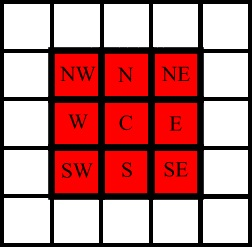
\includegraphics[width=0.33\textwidth, natwidth=252, natheight=247]{Moore_Neighbourhood.jpg}
\end{figure}

Finally, we identify fingertips in the image.  Fingertip candidates are all points appearing on both the convex hull and the contour.  In addition to the actual fingertips, the set of candidates will contain points along the wrist and palm.  To eliminate them, we score each candidate by taking the points eight spots to the left and right along the contour from each candidate, and considering the angle they form with the candidate point.  Candidates with an angle greater than $\pi/3$ are removed.  There may also be several candidate points on the same fingertip; in this case we take the candidate with the best score (i.e. lowest angle).  If we identify the same number of fingertips in four consecutive frames, we recognize it as a gesture.

\begin{figure}
\caption{Fingertip Identification}
\centering
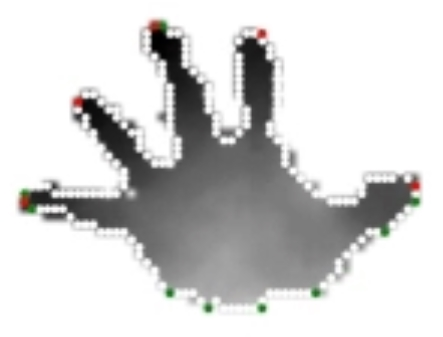
\includegraphics[width=0.5\textwidth, natwidth=443, natheight=337]{Fingertip_Identification.jpg}\\
Green points are the convex hull,\\
white points are the contour, and\\
red points are the fingertips.
\end{figure}



\section{Results}
We found that our implementation of the hand tracking and gesture recognition algorithms operated smoothly at 30 frames per second, and were successful in ordinary playing conditions.  A video demonstration is available at \href{http://youtu.be/GUCRyYfLES4}{http://youtu.be/GUCRyYfLES4}.

One limitation of our algorithm is that segmentation by volume is quite naive.  If the hands are held near the body or other objects, then those objects will be included in the segmentation volume and treated as part of the hand.  To handle these cases, we need to filter out all unconnected pixels in the volume.

A second limitation is that we do not take advantage of depth data when identifying fingertips, so our algorithms begin to fail when the hand is held nearly horizontally.  Making better use of depth data could potentially increase our accuracy.  For example, a promising technique in \cite{Lia12} treats the depth image pixels as nodes in a graph, with the relative depth as the cost between nodes, and examines path lengths along the hand to identify fingertips.



\section{Future Work}
In addition to addressing the limitations above, we think there many ways to continue to enhance the virtual theremin.  The performer's hands still have many degrees of freedom which could control other options.  For example, the pitch hand could move toward and away from the camera to control a vibrato effect, or flick up and down to synthesize attacks on the current pitch.

Another line of work involves synthesizing more than one voice at once.  Using the Microsoft Kinect, we are also able to identify up to four different ``players", so we could implement a multiplayer mode where several people perform together.  We could also implement a recording mode that allowed a single performer to record and play back tracks, performing on top of them.

Finally, we would like to try virtualizing other instruments.  A trumpet, for example, has only a few options for finger configurations which should be quite recognizable using the algorithms we have already implemented (the second hand could indicate the tightness of the embouchure).  Given an accurate enough camera, we fully intend to implement a rockin' air guitar.



\begin{thebibliography}{9}

\bibitem{Rah11}
\textsc{Jagdish L. Raheja, Ankit Chaudhary, and Kunal Singal}:
Tracking of Fingertips and Centres of Palm using KINECT.
In \textit{Third International Conference on Computational Intelligence, Modelling \& Simulation (CIMSiM'11)},
pp.~248-252.
IEEE, 2011.

\bibitem{Li12}
\textsc{Yi Li}:
Hand Gesture Recognition Using Kinect.
In \textit{Third International Conference on Software Engineering and Service Science (ICSESS'12)},
pp.~196-199.
IEEE, 2012.

\bibitem{And79}
\textsc{A.M. Andrew}:
Another efficient algorithm for convex hulls in two dimensions.
In \textit{Information Processing Letters},
vol.~9, no.~5, pp.~216-219.
1979.
http://dx.doi.org/10.1016/0020-0190(79)90072-3

\bibitem{Gra72}
\textsc{R.L. Graham}:
An Efficient Algorithm for Determining the Convex Hull of a Finite Planar Set.
In \textit{Information Processing Letters},
vol.~1, no.~4, pp.~132-133.
1972.

\bibitem{Lia12}
\textsc{Hui Liang, Junsong Yuan, and Daniel Thalmann}:
3D Fingertip and Palm Tracking in Depth Image Sequences.
In \textit{Proceedings of the 20th ACM International Conference on Multimedia (MM'12)},
pp.~785-788
ACM, 2012.

\end{thebibliography}


\newpage
\appendix
\section{Algorithms}

\subsection{Segmentation by Volume}
\begin{small}
\begin{alltt}
\textbf{define} \textit{DepthPoint[]} HandImage(\textit{SkeletonPoint} handJoint,
                              \textit{DepthPoint[]} Image) \textbf{as}
    \textbf{for} depthPoint \textbf{in} Image \textbf{do}
        skeletonPoint \(\leftarrow\) MapToSkeletonSpace(depthPoint)
        \textbf{if} |skeletonPoint.X - handJoint.X| < 15cm \textbf{and}
           |skeletonPoint.Y - handJoint.Y| < 15cm \textbf{and}
           |skeletonPoint.Z - handJoint.Z + 10cm| < 15cm
        \textbf{then}
            yield depthPoint
\end{alltt}
\end{small}


\subsection{Monotone Chain Algorithm}
\begin{small}
\begin{alltt}
\textbf{define} \textit{bool} RightTurn(\textit{Point} a, \textit{Point} b, \textit{Point} c) \textbf{as}
    v1 \(\leftarrow\) (b.X - a.X, b.Y - a.Y)
    v2 \(\leftarrow\) (c.X - a.X, c.Y - a.Y)
    cross \(\leftarrow\) v1.X \(\times\) v2.Y - v1.Y \(\times\) v2.X
    \textbf{if} cross >= 0 \textbf{then}
        \textbf{return} True
    \textbf{else}
        \textbf{return} False

\textbf{define} \textit{Point[]} ConvexHull(\textit{Point[]} points) \textbf{as}
    h \(\leftarrow\) \textit{Point[]}
    n \(\leftarrow\) 0
    points \(\leftarrow\) points.OrderBy(X)
    \textbf{for} p \textbf{in} points \textbf{do}
        \textbf{while} n >= 2 \textbf{and} RightTurn(h[n-2], h[n-1], p) \textbf{do} n--
        h[n++] \(\leftarrow\) point
    min \(\leftarrow\) n + 1
    \textbf{for} p \textbf{in} points.Reverse() \textbf{do}
        \textbf{while} n >= min \textbf{and} RightTurn(h[n-2], h[n-1], p) \textbf{do} n--
        h[n++] \(\leftarrow\) point
    \textbf{return} h.Take(n - 1)
\end{alltt}
\end{small}


\newpage
\subsection{Moore Neighbourhood Tracing}
\begin{small}
\begin{alltt}
\textbf{define} \textit{Point[]} Neighbourhood(\textit{Point} center, \textit{Point} start) \textbf{as}
    x \(\leftarrow\) start.X
    y \(\leftarrow\) start.Y
    \textbf{for} i \textbf{in} [0,8)
        dx \(\leftarrow\) x - center.X
        dy \(\leftarrow\) y - center.Y
        \textbf{if} dx + dy != 0 \textbf{then} x \(\leftarrow\) x - dy
        \textbf{if} dx - dy != 0 \textbf{then} y \(\leftarrow\) y + dx
        \textbf{if} x \textbf{in} [0, Width) and y \textbf{in} [0, Height) \textbf{then}
            \textbf{yield} \textit{Point}(x, y)

\textbf{define} \textit{Point[]} Contour(\textit{Point[]} points) \textbf{as}
    first \(\leftarrow\) points.First(HasDepth)
    current \(\leftarrow\) first
    previous \(\leftarrow\) (current.X - 1, current.Y - 1)
    \textbf{do}
         \textbf{yield} current
         neighbourhood \(\leftarrow\) Neighbourhood(current, previous)
         previous \(\leftarrow\) current
         current \(\leftarrow\) neighbourhood.First(HasDepth)
    \textbf{until} current = first \textbf{or not} HasDepth(current)
\end{alltt}
\end{small}


\newpage
\subsection{Fingertip Identification}
\begin{small}
\begin{alltt}
\textbf{define} \textit{decimal} Score(\textit{Point} candidate, \textit{Point[]} contour) \textbf{as}
    index \(\leftarrow\) contour.IndexOf(candidate)
    left \(\leftarrow\) contour[index - 8 \% contour.Length]
    right \(\leftarrow\) contour[index + 8 \% contour.Length]
    v1 \(\leftarrow\) Normalize(left - candidate)
    v2 \(\leftarrow\) Normalize(right - candidate)
    \textbf{return} ArcCos(DotProduct(v1, v2))

\textbf{define} \textit{Point[]} Fingertips(\textit{Point[]} hull, \textit{Point[]} contour) \textbf{as}
    candidates \(\leftarrow\) hull.Intersect(contour)
                      .Where(Score(candidate) < \(\pi\) / 3)
                      .OrderBy(Score(candidate))
    \textbf{while not} candidates.Empty() \textbf{do}
        finger \(\leftarrow\) candidates.First()
        \textbf{yield} finger
        candidates \(\leftarrow\) candidates.Where(|finger - candidate| > 20)
\end{alltt}
\end{small}

\end{document}
